\section{Einleitung}

\begin{equation}
	M = m \frac{V_m}{V}\frac{p_0}{p}\frac{T}{T_0} \label{eq:dampfMolMasse}
\end{equation}

\section{Versuchsteil}
\subsection{Messung der molaren Masse anhand von Dampfdichte}
Im ersten Versuchsteil wird die molare Masse von Ethanol und Cyclohexan bestimmt. Dazu wird genutzt, dass das molare Volumen von idealen Gasen eine konstante ist und sowohl Ethanol als auch Cyclohexan nur geringfügig von diesem Wert abweichen. \\
Es werden geringe Probenmengen von etwa \SI{.1}{\milli\liter} bei Ethanol und \SI{.2}{\milli\liter} bei Cyclohexan mit einer Spritze in einen Glaskolben injiziert. Durch wiegen der Spritze vorm Injizieren und danach wird die Masse des injizierten Stoffes bestimmt. Die Temperatur des Kolbens wird durch ein kochendes Wasserbad konstant auf etwa \SI{100}{\degreeCelsius} gehalten. Da die Siedepunkte von Ethanol und Cyclohexan, wie Tabelle \ref{tab:propEthanolCyclo} entnommen werden kann, deutlich darunter liegen, gehen diese im Kolben in die gasförmige Phase über. Das so verdrängte Volumen kann abgelesen werden und zusammen mit der Probenmasse die Molmasse bestimmt werden. Durch fünf Messungen pro Stoff wird die Unsicherheit verringert.
\begin{figure}[H]
\centering
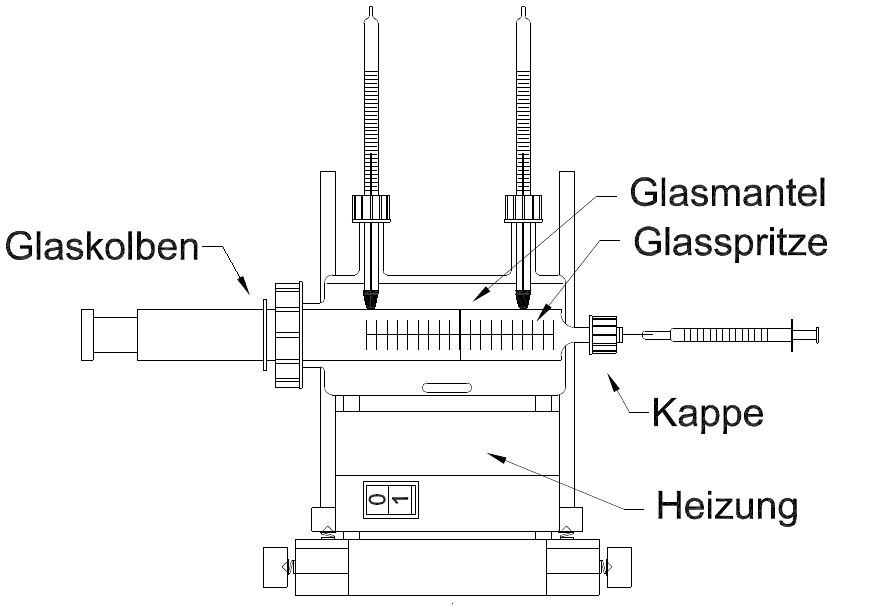
\includegraphics[width=.7\textwidth]{Bilder/aufbau_dampf.png}
\caption[Aufbau]{Versuchsapperatur (Quelle: \cite{anleitung2015})}
\label{fig:aufbau_dampf}
\end{figure}
\subsubsection{Auswertung}

Mit \eqref{eq:dampfMolMasse} lässt sich aus den erfassten Messwerten die molare Masse bestimmen. Da die Formel nur aus linearen und antiproportionalen Zusammenhängen besteht, lässt sich Fehlerformel \eqref{eq:err} verwenden. Der Innendruck des Kolbens passt sich dem Umgebungsdruck an. Daher entspricht $ p $ dem gemessenen Umgebungsdruck $ p = \SI{1001,9(1)}{\hecto\pascal} $. Die Innentemperatur $ T $ war über die Dauer des Experimentes konstant und wurde an beiden Enden gemessen. Die mittlere Temperatur ist $ T = \SI{102,5(8)}{\degreeCelsius} $. Als molares Volumen wird das molare Volumen des idealen Gases von $ V_m = \SI{22.413996(39)}{\mol\per\l} $ angenommen. Dieses gilt bei Normalbedingungen von $ p_0 = \SI{1013,25}{\hecto\pascal} $ und $ T_0 = \SI{0}{\degreeCelsius} $. Die damit bestimmten Ergebnisse sind in den Tabellen \ref{tab:dampf_ethanol} und \ref{tab:dampf_cyclo} zu finden. \\
Die Mittelwerte der molaren Massen betragen \SI{48,3\pm11,7}{\g\per\mol} für Ethanol und \SI{91,9 \pm 15}{\g\per\mol} für Cyclohexan.

\begin{table}[H]
	\centering
	\begin{tabular}{
			S[
				table-figures-integer  = 1,
				table-figures-decimal  = 2
			]|
			S[
				table-figures-integer  = 0,
				table-figures-decimal  = 4
			]|
			S[
			table-figures-integer  = 2,
			table-figures-decimal  = 1
			]}
		{Probenmasse [\si{\g}]} & {Gasvolumen [\si{\l}]} & {Molvolumen [\si{\g\per\mol}]} \\\hline
		0,10 \pm 0,02 & 0,0625 \pm 0,0005 & 49,9 \pm 10,0 \\
		0,13 \pm 0,02 & 0,0825 \pm 0,0005 & 49,1 \pm 7,6 \\
		0,09 \pm 0,02 & 0,0635 \pm 0,0005 & 44,2 \pm 9,9 \\
		0,08 \pm 0,02 & 0,0520 \pm 0,0005 & 48,0 \pm 12,0 \\
		0,13 \pm 0,02 & 0,0805 \pm 0,0005 & 50,3 \pm 7,8 \\
	\end{tabular}
	\caption{Ergebnisse vom ersten Versuch mit Ethanol}
	\label{tab:dampf_ethanol}
\end{table}

\begin{table}[H]
	\centering
	\begin{tabular}{
			S[
				table-figures-integer  = 1,
				table-figures-decimal  = 2
			]|
			S[
				table-figures-integer  = 0,
				table-figures-decimal  = 4
			]|
			S[
				table-figures-integer  = 2,
				table-figures-decimal  = 1
			]}
		
		{Probenmasse [\si{\g}]} & {Gasvolumen [\si{\l}]} & {Molmasse [\si{\g\per\mol}]} \\\hline
		0,24 \pm 0,02 & 0,0765 \pm 0,0005 & 97,8 \pm 8,2 \\
		0,25 \pm 0,02 & 0,0870 \pm 0,0005 & 89,6 \pm 7,2 \\
		0,22 \pm 0,02 & 0,0785 \pm 0,0005 & 87,4 \pm 8,0 \\
		0,14 \pm 0,02 & 0,0510 \pm 0,0005 & 85,6 \pm 12,3 \\
		0,17 \pm 0,02 & 0,0535 \pm 0,0005 & 99,1 \pm 11,7 
		
	\end{tabular}
	\caption{Ergebnisse vom ersten Versuch mit Cyclohexan}
	\label{tab:dampf_cyclo}
\end{table}

\begin{figure}
\centering
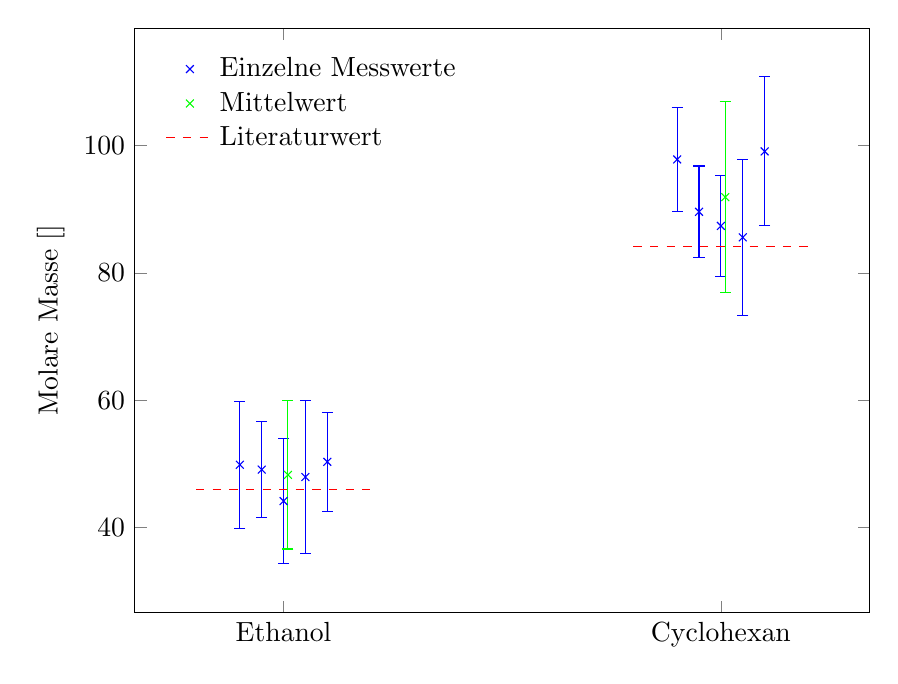
\begin{tikzpicture}
\begin{axis}[width = .9\textwidth, height = 9cm,
	xtick={.3,1.3},
	xticklabels={Ethanol, Cyclohexan},
	ylabel = {Molare Masse [\si{\g\per\mol}]},
	legend style={draw=none, legend cell align = left}, legend pos = north west]

\addplot[blue, only marks, error bars/y dir = both, error bars/y explicit, mark = x] table[x=x,y=y, y error = err] {
x	y	err
.2	49.8785358849	9.9841273896
.25	49.1228004927	7.5637826811
.3	44.1837424177	9.8251242482
.35	47.9601306586	11.9992384215
.4	50.343242741	7.7520048157
};

\addplot[green, only marks, error bars/y dir = both, error bars/y explicit, mark = x] table[x=x,y=y, y error = err] {
x	y	err
.31	48.297690439	11.634048942
};

\addplot[dashed, red, domain=.1:.5] {46.07};

\legend{Einzelne Messwerte, Mittelwert, Literaturwert}

\addplot[blue, only marks, error bars/y dir = both, error bars/y explicit, mark = x] table[x=x,y=y, y error = err] {
x	y	err
1.2	97.8010507547	8.1771956813
1.25	89.5807038163	7.1869095787
1.3	87.3668622188	7.9636160815
1.35	85.5759194104	12.2549480494
1.4	99.0578399583	11.6920686252
};

\addplot[green, only marks, error bars/y dir = both, error bars/y explicit, mark = x] table[x=x,y=y, y error = err] {
x	y	err
1.31	91.8764752317	14.9681458409
};
\addplot[dashed, red, domain=1.1:1.5] {84.16};
\end{axis}
\end{tikzpicture}
\caption{Grafische Darstellung}
\end{figure}


\begin{table}[H]
\centering
\begin{tabular} {c|c|c}
	 & Siedepunkt & Molare Masse \\\hline
	Ethanol & \SI{78,32}{\degreeCelsius} & \SI{46,07}{\g\per\mol} \\
	Cyclohexan & \SI{81}{\degreeCelsius} & \SI{84,16}{ \g\per\mol}
\end{tabular}
\caption{Stoffeigenschaften von Ethanol und Cyclohexan (Quellen: \cite{wiki:cyclohexan}, \cite{wiki:ethanol})}
\label{tab:propEthanolCyclo}
\end{table} 



\section{Diskussion} % !!!!